% %!TEX root = main.tex
\section{Image calibration network}
\label{sec:proposed_method}

In this section, we present our CNN architecture for single image calibration  and compare it to the state-of-the-art estimation method.  To train this model, we need a large number of images and their corresponding camera parameters. However, no such dataset currently exist. Structure from Motion (SfM) datasets~\cite{Wilson2014} provides relatively accurate field of view values but no horizon lines, and conversely the Horizon Lines in the Wild (HLW) dataset~\cite{Workman2016} provides horizon lines but no field of view. In the following, we discuss how we generate our camera calibration dataset, how the CNN model was trained, and we use guided backpropagation to analyze the image features the model focuses on to provide its estimations, which gives insights into the cues that are important to perform camera calibration.

\subsection{Dataset}
\label{sec:dataset_generation}

\begin{table}[!t]
\centering
\footnotesize
\begin{tabular}{lll}
\toprule
Parameter & Distribution & Values \\
\midrule
Focal length (mm) & Lognormal & $\mu=14, \sigma=17$ \\
Horizon (pixels) & Normal & $\mu=0.046, \sigma=0.3$ \\
Roll ($^\circ$) & Cauchy & $x_0 = 0$, $\gamma \in \{0.001, 0.1\}$ \\
Aspect ratio & Varying & $\{1{:}1, 5{:}4, 4{:}3, 3{:}2, 16{:}9\}$ \\
\bottomrule
\end{tabular}
\vspace{1em}
\label{tab:parameters-sampling}
\caption{Sampling of camera parameters used to generate the dataset for the human sensitivity study. }
\end{table}

Our goal is to train a deep network to estimate the camera roll, pitch, and field of view from a single image. To obtain images and their ground truth camera parameters, we take inspiration from \cite{Workman2016,Hold-Geoffroy2017} and leverage the SUN360 database~\cite{Xiao2012}, which contains a large number of $360^\circ$ panoramas. We extract 7 rectified images from each panorama using a standard pinhole camera model of random parameters. To obtain reasonable camera parameters, the sampling strategies indicated in table~\ref{tab:parameters-sampling} were employed. Note that for the camera roll, two different Cauchy distributions are sampled with 0.33 and 0.66 probability respectively. This was done to model the fact that many photos typically have a roll close to 0. The aspect ratios were chosen by sampling Flickr and ImageNet images. Note that a larger probability (0.66) was given to the $4{:}3$ aspect ratio as it is the most common. The other aspect ratios are given a probability of $0.11$. We resize the extracted images to $224\times224$ to fit the neural network input size. This results in a dataset of 399,728 pairs of photos and their corresponding camera calibration which we split into a training set of 389,760 pairs, a validation set of 9,078 pairs and a test set of 890 pairs. Special care was taken to ensure no panorama used in the training set was present in validation or test set through other cropped photos.

As in~\cite{Workman2016}, we use the slope/offset ($\psi,\rho$) representation, where the horizon line is parameterized by the roll $\psi$ and its perpendicular distance from the center of the image $\rho$.

\subsection{Architecture}

We adopt a DenseNet~\cite{Huang2016} model pretrained on ImageNet~\cite{Russakovsky2015} on which we replace the last layer with three separate heads: one for estimating the horizon angle $\psi$, a second one to estimate the horizon's distance to the center of the image $\rho$ and a third one to estimate the vertical field of view of the image $h_{\theta}$.
All output layers use the softmax activation function to output a probability distribution by discretizing their respective parameter into 256 bins. This type of representation was also used in~\cite{Workman2016}. We found that fitting a standard distribution to the CNN output gives a sense of the uncertainty of the estimation, which is not possible to obtain when performing a regression. We adopt a range of $\left[ -\nicefrac{\pi}{2}, \nicefrac{\pi}{2} \right]$ for slope and $\left[ -1.6, 1.6\right]$ for offset. For both parameters, we use smaller bins around 0 for finer estimations around those values. Bin width follow an inverse normal distribution with $\mu=0,\, \sigma=\left\{ 0.5, 1 \right\}$ for slope and offset, respectively. We sum the Kullback-Leibler divergence of the three heads and use it as loss to train the model, which we minimize using stochastic gradient descent with the Adam optimizer~\cite{Kingma2015} with an initial learning rate of $\eta = 0.001$ and a learning rate decay of $ \alpha = 0.0002$. Training is performed on mini-batches of 42 images. Convergence is observed through early stopping typically after 9-10 epochs, presumably because of the large size of our training set and our use of transfer learning through a pretrained model.

\begin{figure}
\centering
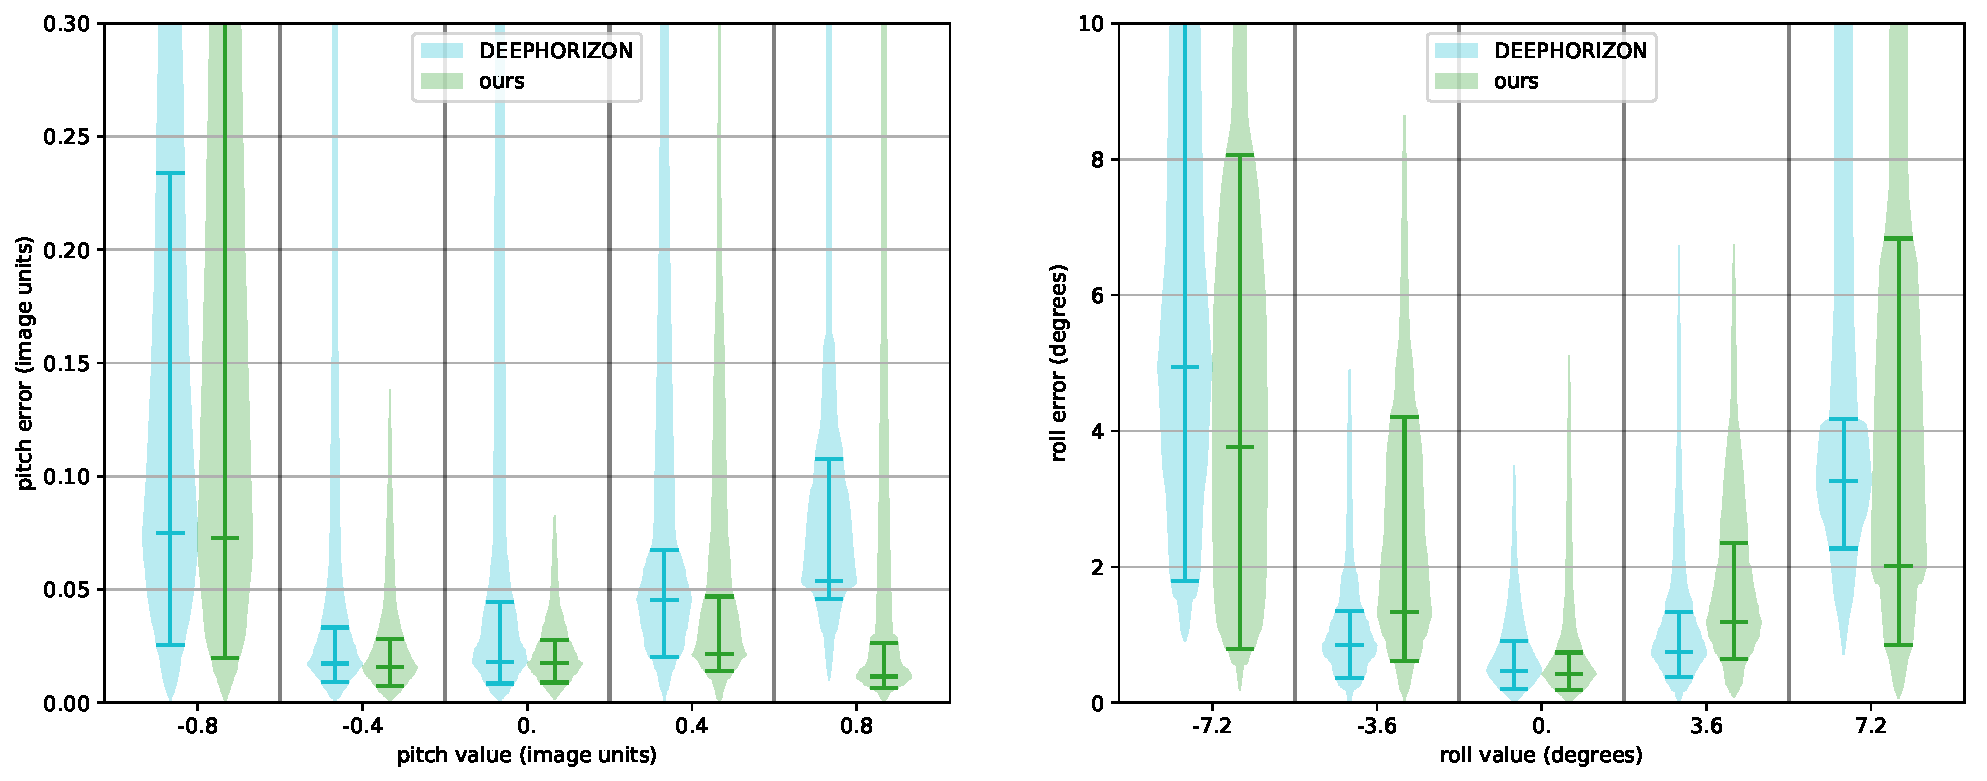
\includegraphics[width=\linewidth]{figures/method/pitch_roll_performance_hlw.pdf} \\
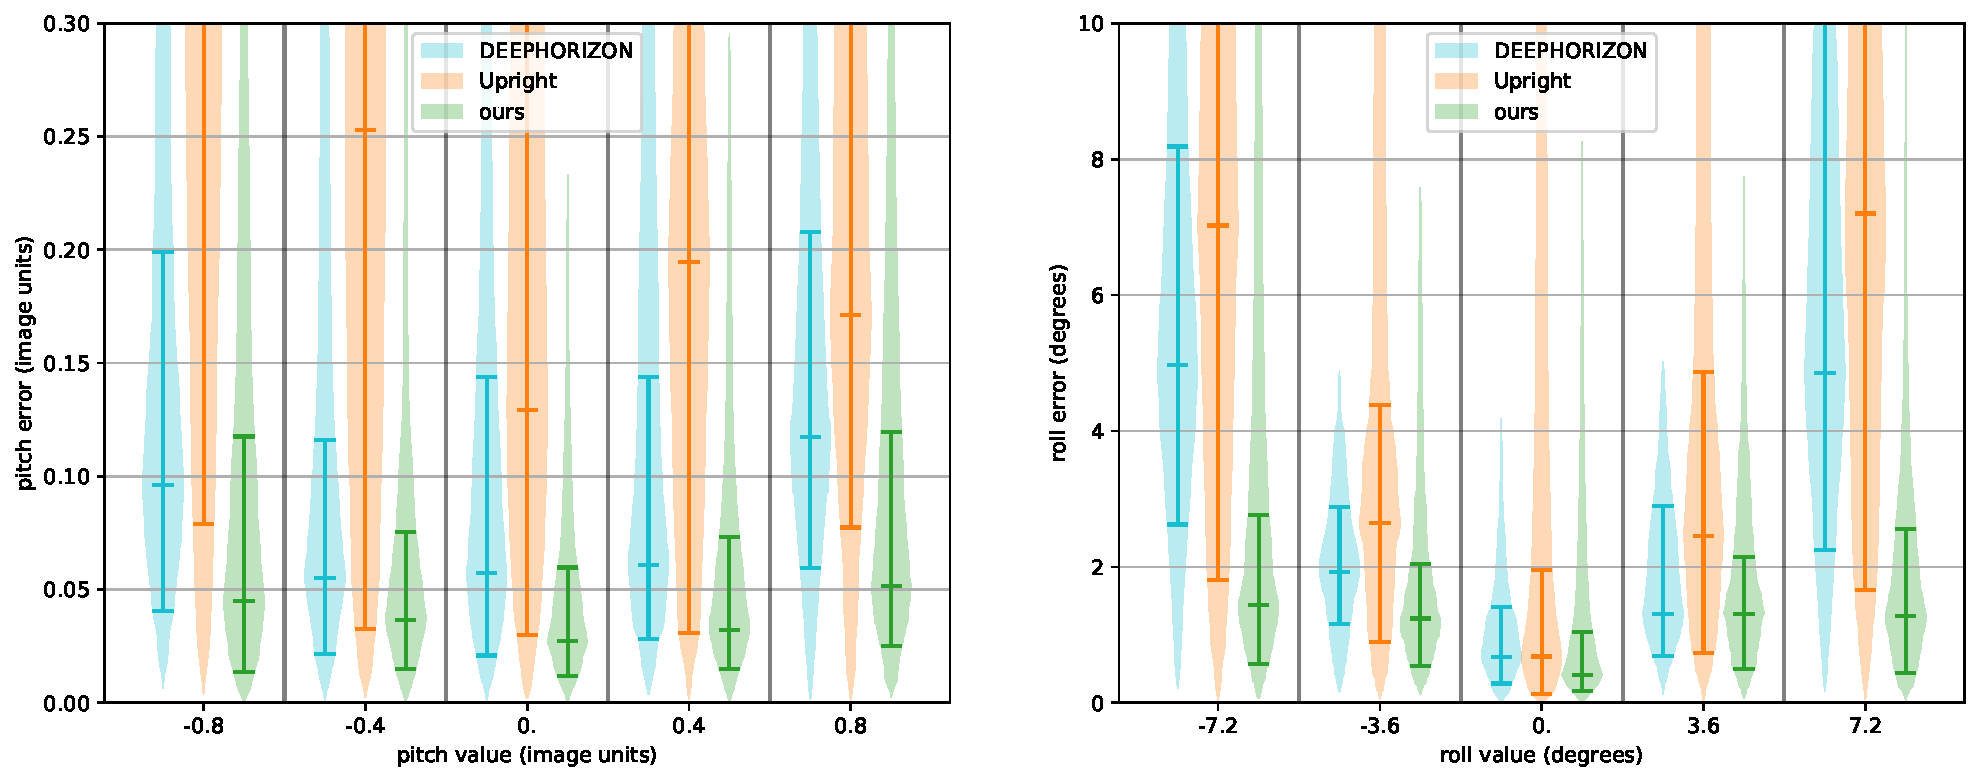
\includegraphics[width=\linewidth]{figures/method/pitch_roll_performance_sun360.pdf}
\caption{Pitch (left) and roll (right) estimation performance on the HLW dataset (top) and our SUN360 test set (bottom). Results are displayed as "box-percentile plots"~\cite{esty-jss-03}, where the envelope of each column represents the percentile and the horizontal bars represents the first quartile, median and third quartile. Estimation errors (y-axis) are grouped into bins according to the parameter value (x-axis).}
\label{fig:method_pitch_roll_performance}
\end{figure}

\begin{figure}
\centering
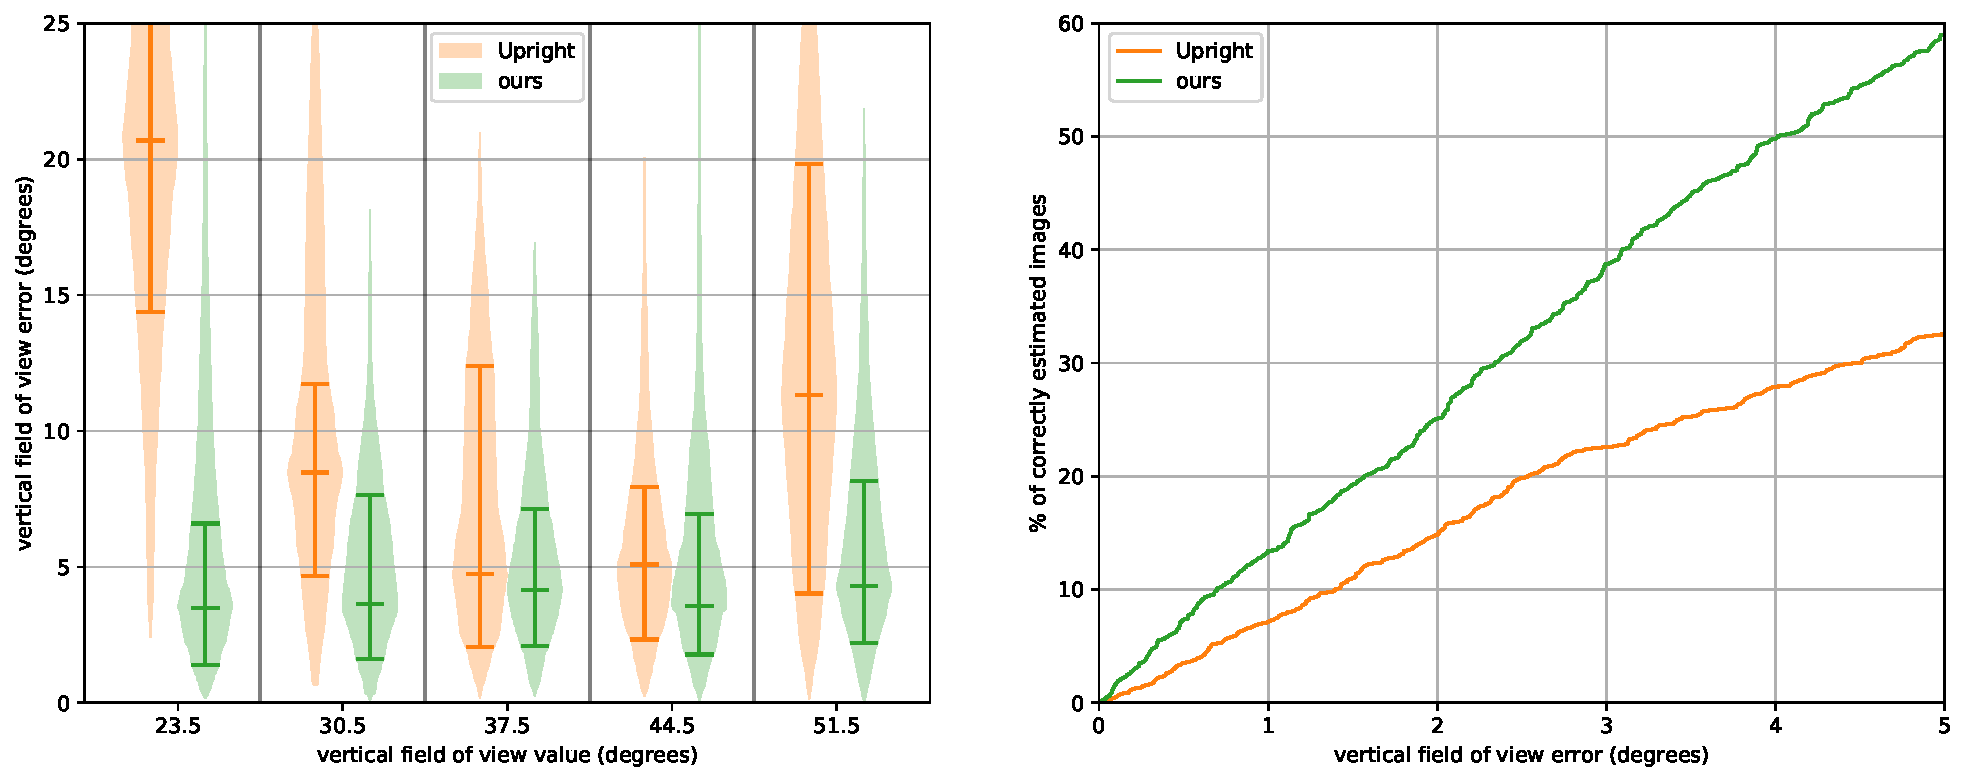
\includegraphics[width=\linewidth]{figures/method/vfov_performance_sun360.pdf}
% \includegraphics[width=\linewidth]{figures/method/vfov_performance_1dsfm.pdf}
\caption{Vertical field of view estimation performance on our SUN360 test set displayed as a "box-percentile plot" (left) and a cumulative distribution function (right). See fig.~\ref{fig:method_pitch_roll_performance} for an explanation of the box plot.
%For the 1DSFM dataset, we also show the performance one would obtain by estimating systematically 38.4\degree, the dataset's median. See fig.~\ref{fig:method_vfov_onedsfm_diversity} for an overview of the diversity of both datasets.
}
\label{fig:method_vfov_performance}
\vspace{-1em}
\end{figure}

% \begin{figure}
% \centering
% \includegraphics[width=\linewidth]{figures/method/vfov_1dsfm_diversity.pdf}
% \caption{Diversity of field of views in our SUN360 test set (left) and the 1DSFM test set (right).}
% \label{fig:method_vfov_onedsfm_diversity}
% \vspace{-1em}
% \end{figure}

\section{Evaluation}

We report quantitative horizon line estimation performance of Upright~\cite{Lee2014}, DEEPHORIZON~\cite{Workman2016} and our method on two different datasets, the Horizon Lines in the Wild (HLW) dataset~\cite{Workman2016} and our SUN360 test set in fig.~\ref{fig:method_pitch_roll_performance}. We observe that aside from large roll errors on HLW, our method outperforms the state-of-the-art in most cases. Upright fails to converge on many cases since multiple images in our SUN360 test set do not contain edges on which the technique relies on. Qualitative results are shown in fig.~\ref{fig:method_example_results}.

Fig.~\ref{fig:method_vfov_performance} shows the quantitative field of view estimation performance on our SUN360 test set.
% and DEEPFOCAL's subset of the 1DSFM dataset~\cite{Workman2015a} 
Our method significantly outperforms Upright~\cite{Lee2014} across the entire range of parameters.
% For the 1DSFM dataset, we also provide the performance when the estimation is always the median of this dataset, 38.4\degree, which puts almost 60\% of the estimations within 5\degree error. We show the diversity of fields of view in both our SUN360 test set and 1DSFM (fig.~\ref{fig:method_vfov_onedsfm_diversity}). Note that no ground truth field of view is available for the HLW dataset and no horizon line annotations are provided with the 1DSFM dataset.



\newcommand{\sgbpwidth}{0.2}
\begin{figure*}
\centering
\bgroup
\def\arraystretch{0}
\begin{tabular}{@{}c@{}c@{}c@{}c@{}c@{}}
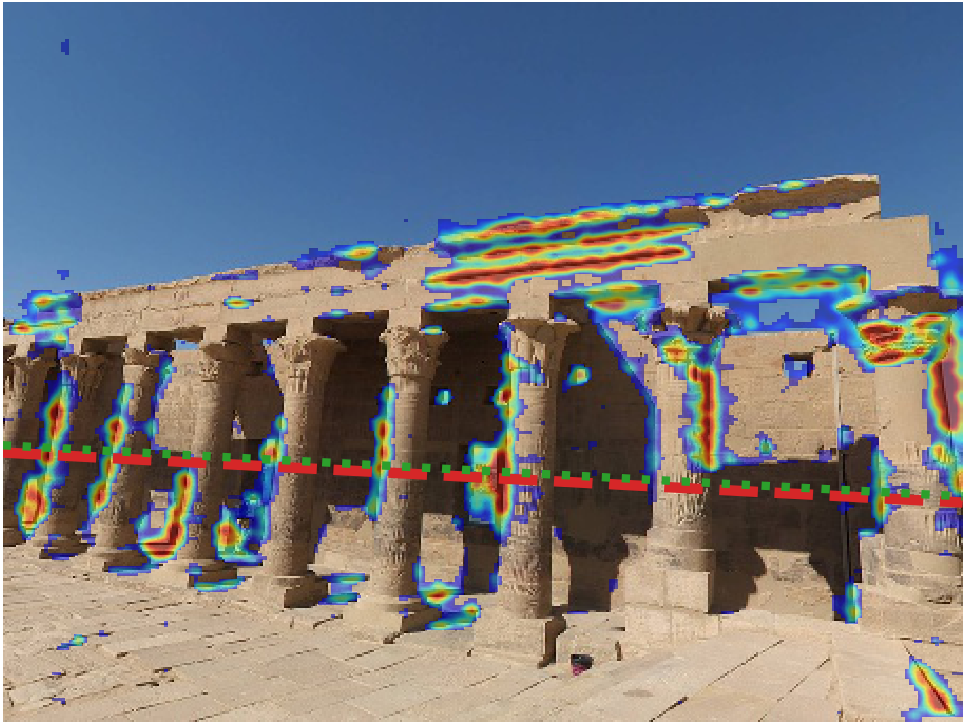
\includegraphics[width=\sgbpwidth\linewidth]{figures/nn_analysis/sgbp/pano_addbhhhqoevobx_jpg-1.png} &
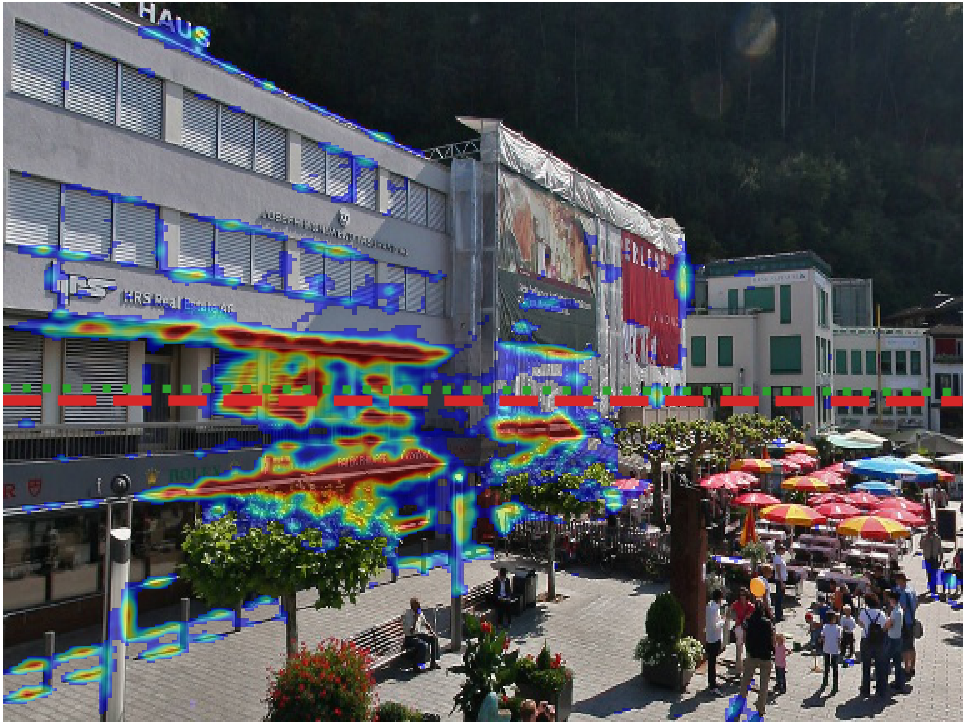
\includegraphics[width=\sgbpwidth\linewidth]{figures/nn_analysis/sgbp/pano_addfjqyibbzulh_jpg-2.png} &
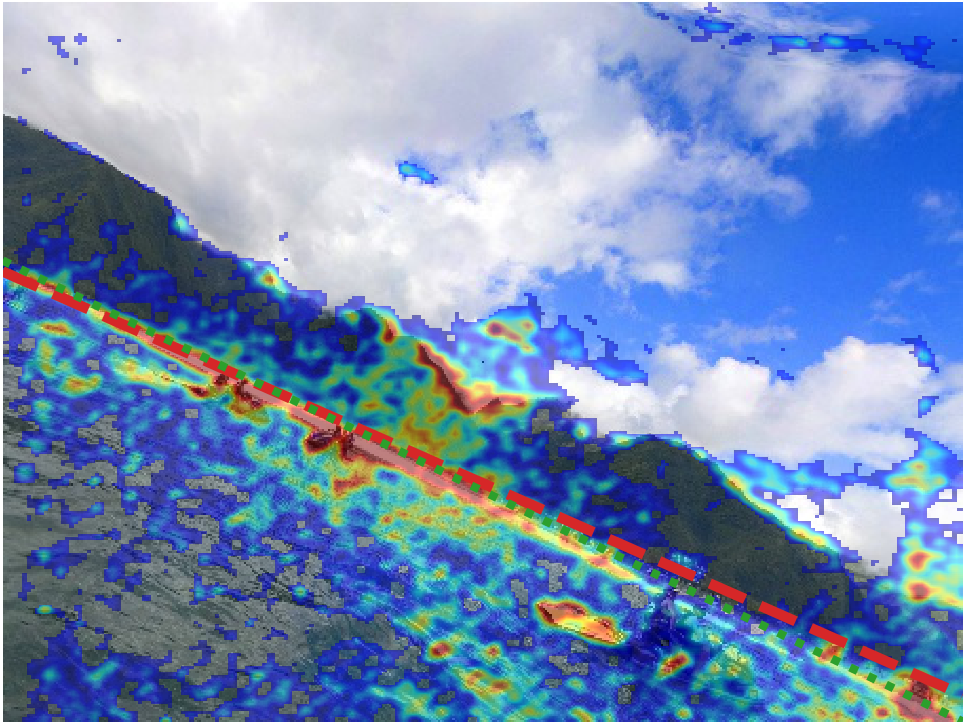
\includegraphics[width=\sgbpwidth\linewidth]{figures/nn_analysis/sgbp/pano_addgasjevqjafh_jpg-1.png} &
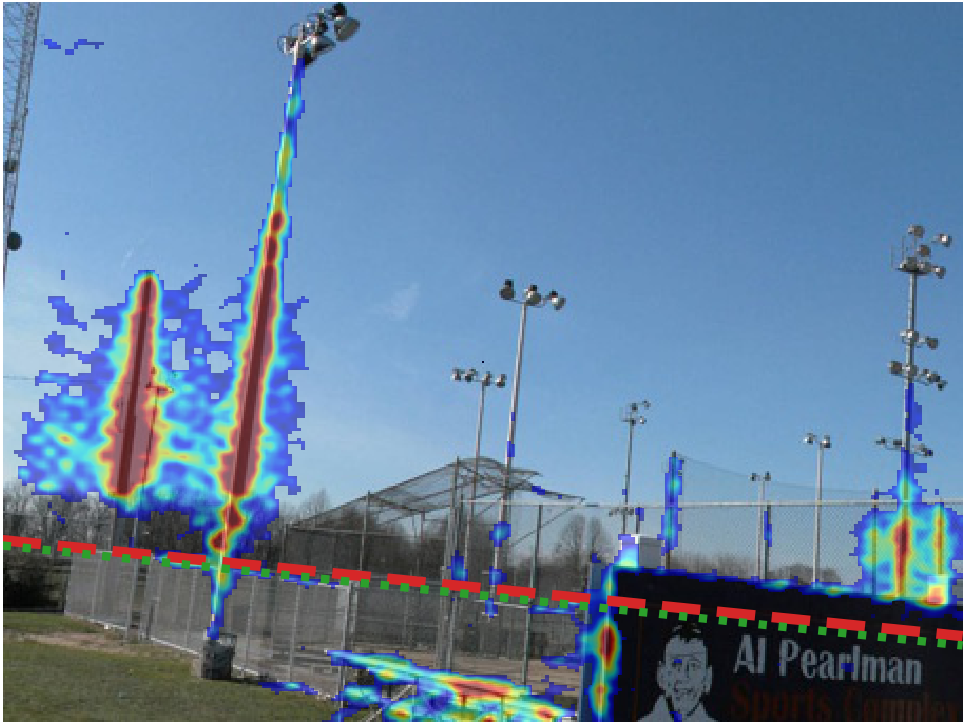
\includegraphics[width=\sgbpwidth\linewidth]{figures/nn_analysis/sgbp/pano_ayfwzaseviqbww_jpg-2.png} &
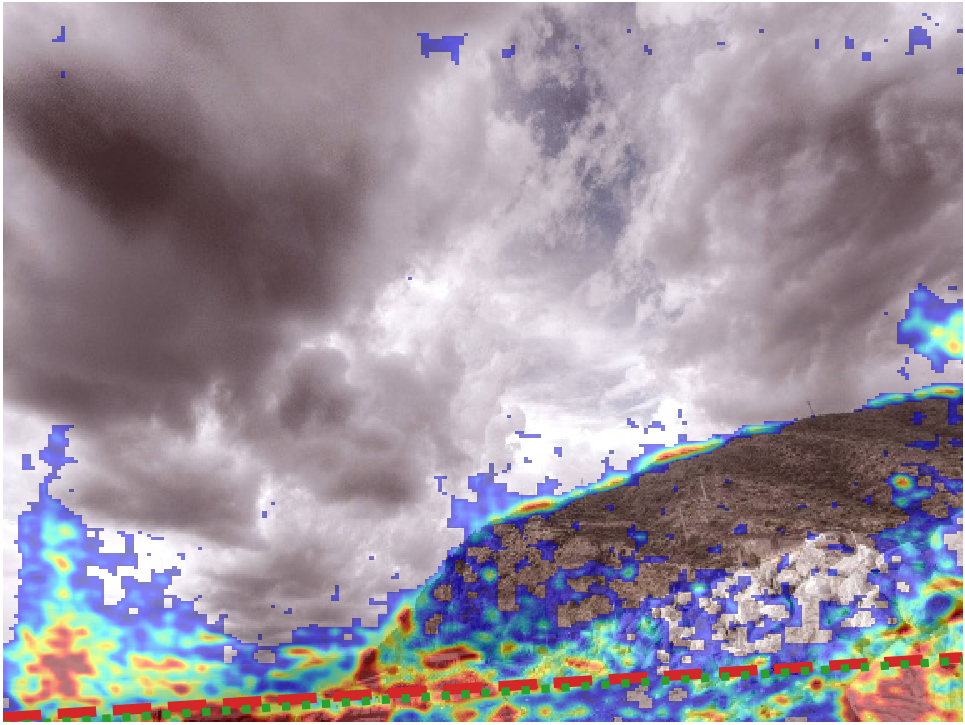
\includegraphics[width=\sgbpwidth\linewidth]{figures/nn_analysis/sgbp/pano_addtfngrqwwyvb_jpg-6.png} \\
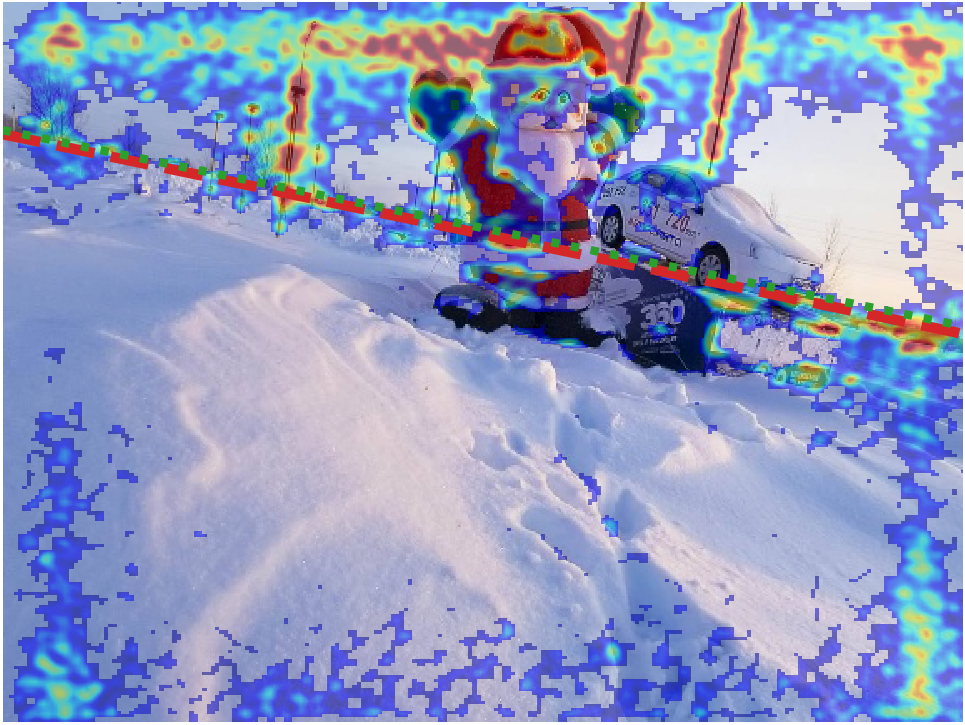
\includegraphics[width=\sgbpwidth\linewidth]{figures/nn_analysis/sgbp/pano_addtwdtklktubg_jpg-3.png} &
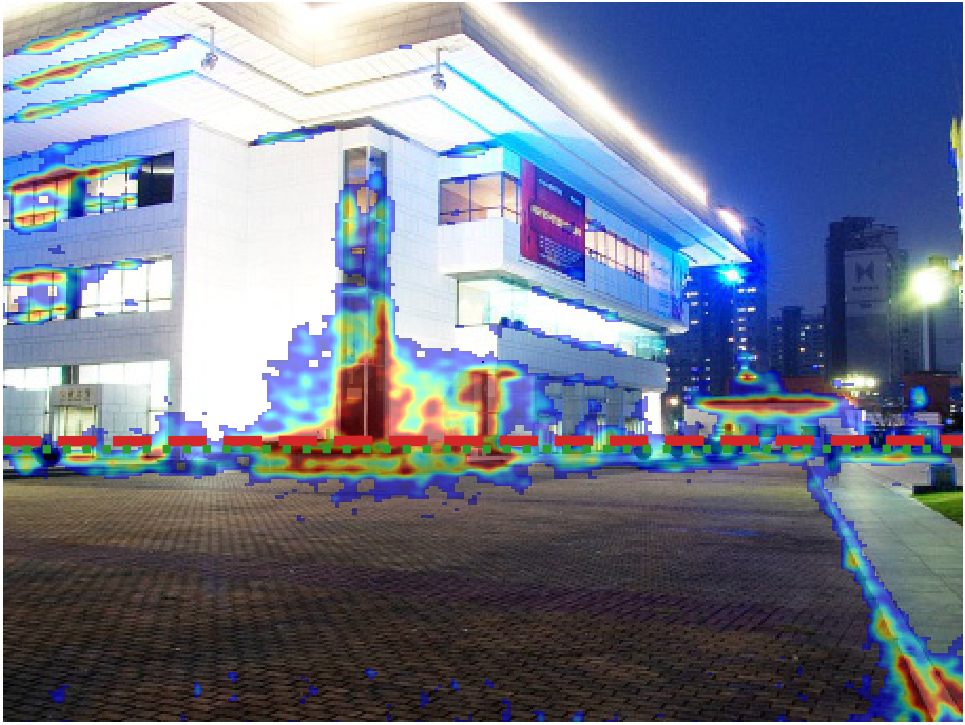
\includegraphics[width=\sgbpwidth\linewidth]{figures/nn_analysis/sgbp/pano_ayflzrhzcccird_jpg-4.png} &
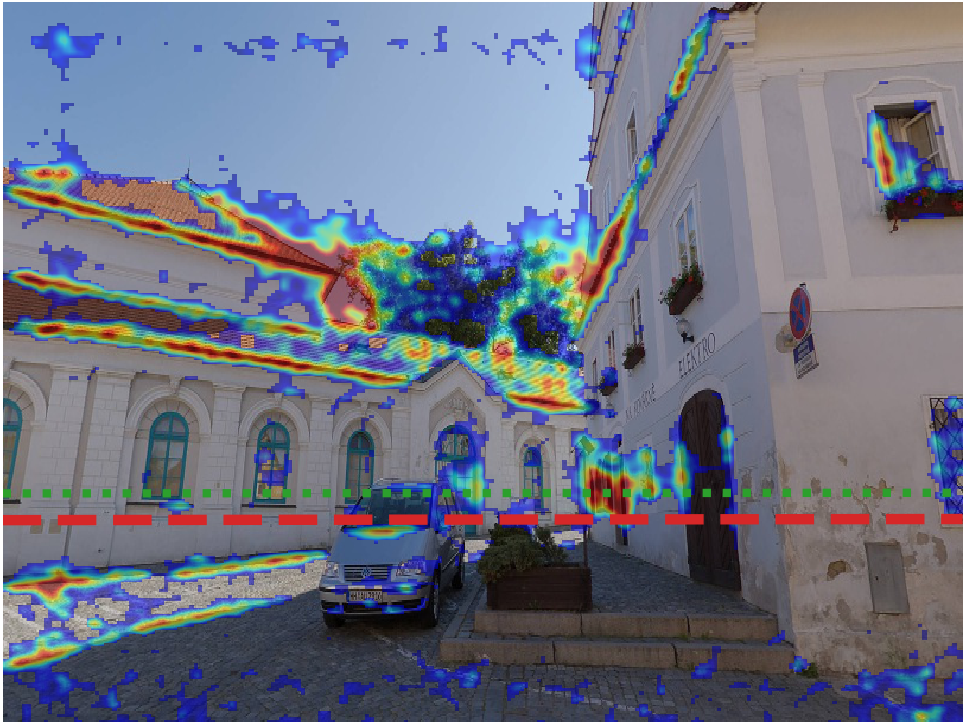
\includegraphics[width=\sgbpwidth\linewidth]{figures/nn_analysis/sgbp/pano_ayfpxlgzfcixnm_jpg-6.png} &
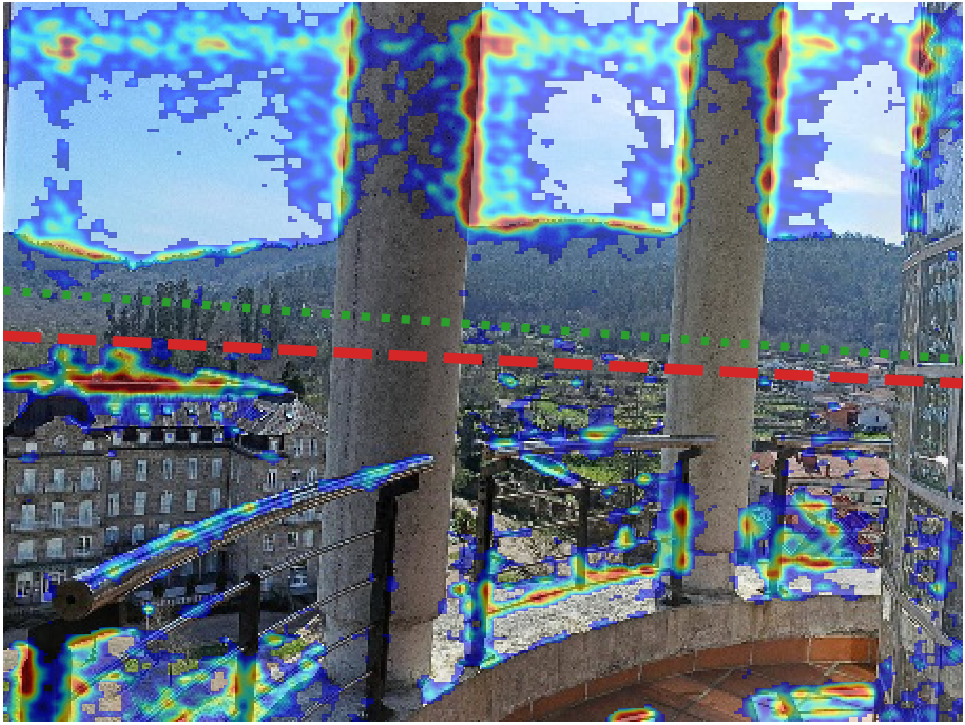
\includegraphics[width=\sgbpwidth\linewidth]{figures/nn_analysis/sgbp/pano_addontedcyafqk_jpg-6.png} &
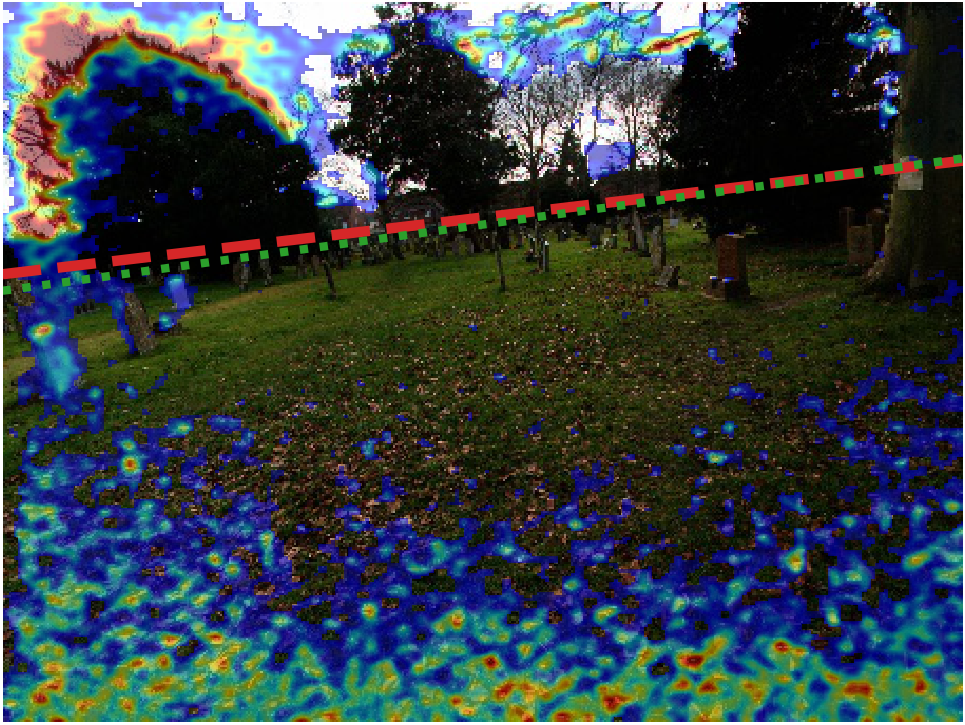
\includegraphics[width=\sgbpwidth\linewidth]{figures/nn_analysis/sgbp/pano_addhxkomphqrlr_jpg-4.png} \\
\multicolumn{5}{@{}c@{}}{
\includegraphics[trim={0 0.5cm 0.5cm 0},clip,width=0.3\linewidth]{figures/nn_analysis/sgbp/sgbp_colorbar.pdf}}
\end{tabular}
\egroup
\def\arraystretch{0.5} % this doesn't seem to do exactly what I want, but it does something
\caption{\textbf{Analysis of the neural network focus.} The result of smoothed guided backpropagation is displayed as a jet overlay. When present, edges corresponding to important vanishing lines are highlighted while other edges are discarded. When no clear horizontal vanishing lines are detected, the neural network seems to look for the boundary between the sky and land while dismissing the clouds. \textbf{More examples available in the supplementary material.}}
\label{fig:nn_analysis_smoothed-guided-back-propagation}
\end{figure*}

\paragraph{Feature analysis} We use guided backpropagation~\cite{Springenberg2015} to understand the image features our CNN-based method focuses on to perform its estimation. We use the smoothgrad~\cite{Smilkov2017} version of guided backpropagation (SGB) to obtain a more stable analysis. Qualitative results are shown in fig.~\ref{fig:nn_analysis_smoothed-guided-back-propagation}. Note how edges representing vanishing lines are highlighted by SGB in accordance to the features used by geometry-based approaches such as Upright. Sharp edges that are not useful for horizon estimation are not taken into account, such as clouds or organic objects. As such, we believe this focus map could help geometric-based approaches select the appropriate edges for geometric calibration estimation. Furthermore, when no clear vanishing line is detected in the image, the CNN model tend to focus on boundaries between sky and land, as the horizon typically lies on or below this boundary.
% YHG: ~\cite{Beardsley1992} <- they detect horizon lines by segmenting the sky, maybe not worth citing


